\section{Design and implementation}
\label{sec: design_implementation}

This section describes the design and implementation of MRDAG-Gen.
MRDAG-Gen iterates over the construction of the graph and the set of properties for all parameter combinations described by the user in the configuration file as shown in the upper right of Fig.~\ref{fig: system_model}.
Section~\ref{ssec: common} shows the common functionalities of MRDAG-Gen, Section~\ref{ssec: graph_construction} describes the three graph generation methods of MRDAG-Gen, and Section~\ref{ssec: set_properties} explains how to set properties for the graph.



\begin{figure}[tb]
    \begin{tabular}{c}
        \begin{minipage}{0.495\linewidth}
            \centering
            \begin{tabular}{l}
                \lstset{linewidth=4.0cm, basicstyle=\scriptsize}
                \lstinputlisting{src/code/combo_exam.txt}
            \end{tabular}
        \end{minipage}
        \hfill
        \begin{minipage}{0.495\linewidth}
            \centering
            \scalebox{0.85}{
                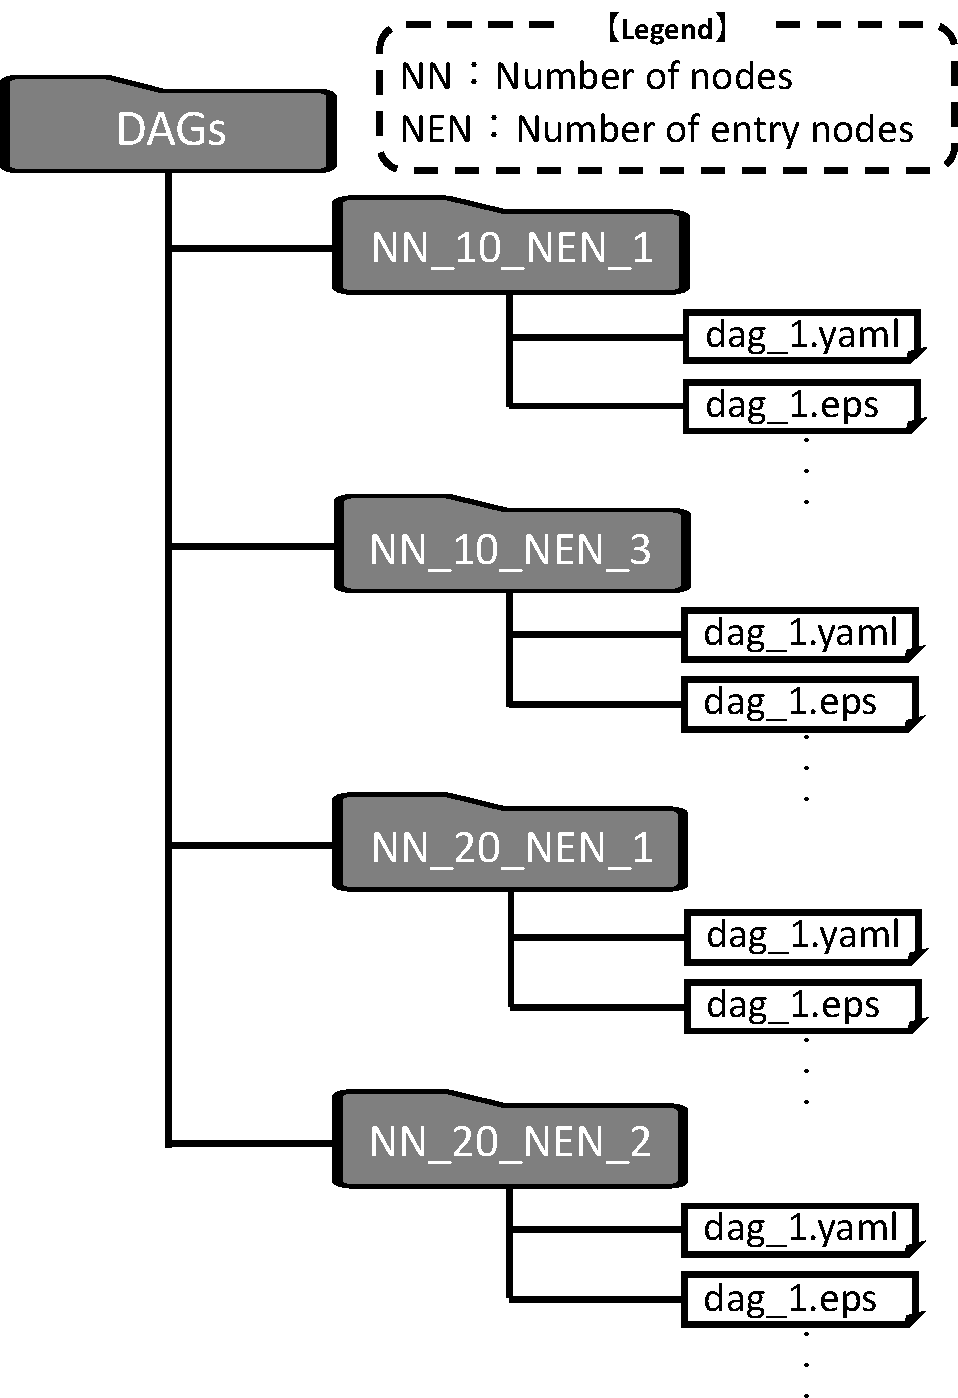
\includegraphics[width=\linewidth]{./src/figure/combination_example.pdf}
            }
        \end{minipage}
    \end{tabular}
    \caption{Example of combination.}
    \label{fig: combo_exam}
\end{figure}


\subsection{Common functionality}
\label{ssec: common}

MRDAG-Gen receives as input a YAML file written by the user, and with a single command, MRDAG-Gen generates all random DAGs with different parameter combinations.
An example of an input parameter file in YAML format is shown on the left side of Fig.~\ref{fig: combo_exam}.
Since MRDAG-Gen allows the user to specify seed values for pseudo-random number generation (line 1 in Fig~\ref{fig: combo_exam}), the same YAML file can be used to easily reproduce random DAG sets generated by other researchers.
    {\it Number of DAGs} (line 2 in Fig~\ref{fig: combo_exam}) is the number of DAGs randomly generated for each combination.
The shape of the generated DAGs is determined by the parameters under {\it Graph structure}, and the properties set for nodes and edges are determined by the parameters under {\it Properties}.

For parameters that require numeric input, users can specify values in the following three ways.
\begin{enumerate}
    \item {\it Fixed}: Only one value is specified, and this value is always used when the DAG is generated. This specification method can be utilized in DAGs where end-to-end deadlines are considered, and one exit node is always desired (line 15 in Fig.~\ref{fig: combo_exam}).
    \item {\it Random}: When a DAG is generated, one is selected at random from the input range. The most basic specification method is used when there is no special intention and to have a variety of values, as shown in lines 9, 11 and 19 in Fig.~\ref{fig: combo_exam}.
    \item {\it Combination}: MRDAG-Gen generates DAGs for all combinations of all lists of parameters for which {\it Combination} is specified. This specification method allows all DAG sets used in random evaluations in DAG studies to be generated in single command execution. Therefore, MRDAG-Gen can significantly reduce the time and effort of researchers using DAGs. For example, when {\it Combination} of {\it Number of nodes} is {\it [10, 20]} and {\it Combination} of {\it Number of entry nodes} is {\it [1, 3],} MRDAG-Gen generates 100 DAGs for all combinations, as shown on the right side of Fig.~\ref{fig: combo_exam}.
\end{enumerate}

When specifying ranges for {\it Random} and {\it Combination} in MRDAG-Gen, the following two intuitive descriptions are possible.
\begin{enumerate}
    \item {\it List format}: The user describes the choices in a list (array) format (such as {\it [10, 20]} in the line 7 in Fig.~\ref{fig: combo_exam})
    \item {\it Tuple format}: The user describes {\it start} value, {\it stop} value, and {\it step} (such as {\it (start=1, stop=3, step=1)} in the line 9 in Fig.~\ref{fig: combo_exam}). The tuple format is internally expanded into a list format of values that are sequentially added to the {\it step} from the {\it start} value to the {\it stop} value (e.g., {\it (start=1, stop=3, step=1)} expands to a list of {\it [1, 2, 3]}). Here, {\it "start="}, {\it "stop="}, and {\it "step="} are optional (line 11 in Fig.~\ref{fig: combo_exam}).
\end{enumerate}

MRDAG-Gen can output DAG description files in YAML, JSON, XML, and DOT formats, and DAG image files in EPS, PDF, SVG, and PNG formats.


\begin{table*}[tb]
    \label{tab: graph_structure}
    \caption{Graph structure}
    \renewcommand{\arraystretch}{1.2}
    \centering
    \scalebox{0.8}{
        \begin{tabular}{l|lll}
            \hline\hline
            \multicolumn{1}{c|}{Generation methods}                                                                   & \multicolumn{2}{c|}{Parameters}                  & \multicolumn{1}{c}{Descriptions}                                                                                                                                                  \\ \hline\hline
            \MC{1}{l|}{\multirow{4}{*}{\begin{tabular}[c]{@{}l@{}}{\it Fan-in/Fan-out}\\ {\it G(n, p)}\end{tabular}}} & \MC{2}{l|}{{\it Number of nodes}}                & Number of nodes in a single DAG                                                                                                                                                   \\ \cline{2-4}
                                                                                                                      & \MC{2}{l|}{{\it Number of entry nodes}}          & Number of entry nodes in a single DAG                                                                                                                                             \\ \cline{2-4}
            \MC{1}{l|}{}                                                                                              & \MC{2}{l|}{{\it Number of exit nodes}}           & Number of exit nodes in a single DAG                                                                                                                                              \\ \cline{2-4}
            \MC{1}{l|}{}                                                                                              & \MC{2}{l|}{{\it Ensure weakly connected}}        & When True is specified, the generated DAGs are always weakly connected                                                                                                            \\ \hline
            \MC{1}{l|}{\MR{2}{{\it Fan-in/Fan-out}}}                                                                  & \MC{2}{l|}{{\it In-degree}}                      & Number of edges input to one node                                                                                                                                                 \\ \cline{2-4}
            \MC{1}{l|}{}                                                                                              & \MC{2}{l|}{{\it Out-degree}}                     & Number of edges output from one node                                                                                                                                              \\ \hline
            \MC{1}{l|}{{\it G(n, p)}}                                                                                 & \MC{2}{l|}{{\it Probability of edge existence}}  & Probability of an edge present between any nodes                                                                                                                                  \\ \hline
            \MC{1}{l|}{\MR{9}{{\it Chain-based}}}                                                                     & \MC{2}{l|}{{\it Number of chains}}               & Number of chains in a single chain-based DAG                                                                                                                                      \\ \cline{2-4}
            \MC{1}{l|}{}                                                                                              & \MC{2}{l|}{{\it Main sequence length}}           & Length of the longest path in a single chain                                                                                                                                      \\ \cline{2-4}
            \MC{1}{l|}{}                                                                                              & \MC{2}{l|}{{\it Number of sub sequences}}        & Number of branches from the main sequence in a single chain                                                                                                                       \\ \cline{2-4}
            \MC{1}{l|}{}                                                                                              & \MC{1}{l|}{\MR{3}{{\it Vertically link chains}}} & \MC{1}{l|}{{\it Number of entry nodes}}                                & Number of entry nodes in a single DAG                                                                    \\ \cline{3-4}
            \MC{1}{l|}{}                                                                                              & \MC{1}{l|}{}                                     & \MC{1}{l|}{{\it Main sequence tail}}                                   & When True is specified, the tail of the main sequence is randomly connected to the head of another chain \\ \cline{3-4}
            \MC{1}{l|}{}                                                                                              & \MC{1}{l|}{}                                     & \MC{1}{l|}{{\it Sub sequence tail}}                                    & When True is specified, the tail of the sub sequence is randomly connected to the head of another chain  \\ \cline{2-4}
            \MC{1}{l|}{}                                                                                              & \MC{1}{l|}{\MR{3}{{\it Merge chains}}}           & \MC{1}{l|}{{\it Number of exit nodes}}                                 & Number of exit nodes in a single DAG                                                                     \\ \cline{3-4}
            \MC{1}{l|}{}                                                                                              & \MC{1}{l|}{}                                     & \MC{1}{l|}{{\it Middle of chain}}                                      & Merge from a tail node of a random chain to a node other than the head and tail of another chain         \\ \cline{3-4}
            \MC{1}{l|}{}                                                                                              & \MC{1}{l|}{}                                     & \MC{1}{l|}{{\it Exit node}}                                            & Merge a head node of a random chain with the exit node.                                                  \\ \hline
        \end{tabular}
    }
\end{table*}


\subsection{Graph construction}
\label{ssec: graph_construction}

MRDAG-Gen extends the {\it Fan-in/Fan-out} \cite{tgff}, {\it G(n, p)} \cite{cordeiro2010random} method widely used in the scheduling field for DAG researchers.
In addition, MRDAG-Gen provides a {\it Chain-based} method for generating state-of-the-art chain-based multi-rate DAGs as shown in Fig~\ref{fig: system_model}.
The parameters that can be specified in {\it Graph structure} of MRDAG-Gen are listed in Table~\ref{tab: graph_structure}.


\begin{table}[tb]
    \centering
    \caption{Helper functions in algorithms}
    \label{tab: helper_functions}
    \renewcommand{\arraystretch}{1.2}
    \scalebox{1.0}{
        \begin{tabular}{c|l}\hline\hline
            Random($a$, $b$) $|$ $a, b \in \mathbb{N}$ & \tabml{Function that returns a random natural     \\ number between $a$ and $b$} \\ \hline
            In($\tau_i$)                               & Function that returns the in-degree of $\tau_i$   \\\hline
            Out($\tau_i$)                              & Function that returns the out-degree of $\tau_i$  \\\hline
            Sequence($\{\tau_i, ..., \tau_k\}$)        & \tabml{Function that returns a straight-line node \\ sequence consisting of a set of input nodes. \\ For example, when the input is $\{\tau_1, \tau_2, \tau_3\}$, \\ return $\{\tau_1, e_{1, 2}, \tau_2, e_{2, 3}, \tau_3\}$.} \\\hline
        \end{tabular}
    }
\end{table}


\begin{algorithm}[t]
    {\footnotesize
        \KwIn{
            $n$ \la {\it Number of nodes} \\
            $nen$ \la {\it Number of entry nodes} \\
            $nex$ \la {\it Number of exit nodes} \\
            $id$ \la {\it In-degree} \\
            $od$ \la {\it Out-degree} \\
        }
        \KwOut{A DAG that satisfies user-specified parameters}
        Initialize $G$ \la $(V, E)$, with $V$ \la $\{\tau_1, ..., \tau_{nen}\}$ and $E$ \la $\{\emptyset\}$ \\
        \While{$|V| \neq n - nex$}{

            \If{Random(0, 1) = 1}{
                \tcc{Fan-in phase}
                $S$ \la Set of nodes in $V$ whose out-degree is less than or equal to $od$ \\
                $r$ \la Random(1, $id$) \\
                $T$ \la Randomly choose $r$ nodes from $S$ \\
                $V$ \la $V \cup \{\tau_{|V|+1}\}$ \\
                \ForEach{$\tau_i$ $\in$ $T$}{
                    $E$ \la $E \cup \{e_{i, |V|}\}$ \\
                }
            }
            \Else{
                \tcc{Fan-out phase}
                $\tau_i$ \la The node with the largest difference between $od$ and its out-degree in $V$ \\
                $diff$ \la $od$ $-$ Out($\tau_i$) \\
                $r$ \la Random(1, $diff$) \\
                \ForEach{k $\in$ $|V|+1$, ... $|V|+m+1$}{
                    $V$ \la $V \cup \{\tau_{k}\}$ \\
                    $E$ \la $E \cup \{e_{i, k}\}$ \\
                }
            }
            \If{$|V| > n - nex$}{
                Initialize $G$ \la $(V, E)$, with $V$ \la $\{\tau_1, ..., \tau_{nen}\}$ and $E$ \la $\{\emptyset\}$
            }
        }
        $G$ \la add\_exit\_nodes($G$, $nex$) \\
        $G$ \la weakly\_connect($G$) \\
        return $G$
        \caption{{\it Fan-in/Fan-out} method in MRDAG-Gen}
        \label{alg: fan_in_fan_out}
    }
\end{algorithm}


\begin{algorithm}[t]
    {\footnotesize
    \KwIn{$G$: A DAG, $nex$: {\it Number of exit nodes}}
    \KwOut{DAG with exit nodes added}
    $X$ \la $\{\tau_{|V|+1}, ..., \tau_{|V|+nex+1}\}$ \\
    $O$ \la Set of current exit nodes of $G$ \\
    \While{$\exists x \in X$, In($\tau_x) = 0$, or $\exists o \in O$, out($\tau_o) = 0$}{
        $\tau_i$ \la The node with the smallest out-degree in $O$ \\
        $\tau_j$ \la The node with the smallest in-degree in $X$ \\
        $E$ \la $E \cup \{e_{i, j}\}$ \\
    }
    $V$ \la $V \cup X$ \\
    return $G$
    \caption{add\_exit\_nodes($G$, $nex$)}
    \label{alg: add_exit_nodes}
    }
\end{algorithm}


\begin{algorithm}[t]
    {\footnotesize
        \KwIn{$G$: A DAG}
        \KwOut{A weakly connected DAG}
        \While{$G$ is not weakly connected}{
            $M$ \la Weakly connected component with the maximum number of nodes in $G$ \\
            $W$ \la Randomly selected a weakly connected component other than $M$ \\
            $\tau_i$ \la Randomly choose one of the exit nodes in $W$ \\
            $\tau_j$ \la Randomly choose one node other than entry nodes in $M$ \\
            $E$ \la $E \cup \{e_{i, j}\}$ \\
        }
        return $G$
        \caption{weakly\_connect($G$)}
        \label{alg: weakly_connect}
    }
\end{algorithm}


\subsubsection{Fan-in/Fan-out method}
\label{sssec: fan_in_fan_out}

{\it Fan-in/Fan-out} is the random DAG generation method proposed by Dick et al. and provided by TGFF \cite{tgff}.
{\it Fan-in/Fan-out} method can specify a range of in-degree (i.e., the number of edges to be input) and out-degree (i.e., the number of edges to be output) for one node, and a DAG is generated in which all nodes satisfy this condition.
    {\it Fan-in/Fan-out} method extends the graph by randomly repeating Fan-in and Fan-out phases.
However, the original {\it Fan-in/Fan-out} method cannot completely satisfy the researcher's requirements.

Since scheduling and allocation methods using DAGs affect performance depending on the number of nodes in a DAG, evaluations are performed with various changes in the number of nodes \cite{senapati2021hmds, tong2020ql}.
However, TGFF does not allow the user to completely control the number of nodes in a DAG to be generated.
In addition, the DAG generated by {\it Fan-in/Fan-out} method has just one entry node, while in-vehicle and self-driving systems have multiple sensors \cite{verucchi2020latency,guanindustry} and require a DAG with multiple entry nodes.
Although the latest version of TGFF allows multiple entry nodes, it may generate DAGs that are not weakly connected.
The number of exit nodes must also be able to be specified since many studies consider DAGs with a single exit node \cite{cho2021conditionally, zhang2020efficient}.

To meet these requirements, MRDAG-Gen allows the specification of the number of nodes, entry nodes, and exit nodes in a single DAG and ensures weakly connected.
The {\it Fan-in/Fan-out} method procedure provided by MRDAG-Gen is shown in Algorithm~\ref{alg: fan_in_fan_out}, and the helper functions used in algorithms are listed in Table~\ref{tab: helper_functions}.
First, the DAG is initialized with a specified number of entry nodes (line 1 in Algorithm~\ref{alg: fan_in_fan_out}).
MRDAG-Gen iteratively expands the graph until the number of nodes fits within a user-specified value (line 2 in Algorithm~\ref{alg: fan_in_fan_out}).
The graph is randomly extended in Fan-in phase or Fan-out phase (lines 3-20 in Algorithm~\ref{alg: fan_in_fan_out}).
If the number of nodes exceeds the user-specified value, the DAG is initialized (lines 21-23 in Algorithm~\ref{alg: fan_in_fan_out}).
After the loop ends, the {\it add\_exit\_nodes} function is called and nodes with no output edges are merged into a user-specified number of exit nodes with the minimum number of edges (Algorithm~\ref{alg: add_exit_nodes}).
Finally, the {\it weakly\_connect} function is called to add edges until the DAG is weakly connected (Algorithm~\ref{alg: weakly_connect}).
With these extensions, MRDAG-Gen's {\it Fan-in/Fan-out} method allows the user to fully control the number of nodes, entry nodes, and exit nodes in one DAG and also guarantees weakly connected.


\begin{algorithm}[t]
    {\footnotesize
        \KwIn{
            $n$ \la {\it Number of nodes} \\
            $p$ \la {\it probability of edge existence} \\
            $nen$ \la {\it Number of entry nodes} \\
            $nex$ \la {\it Number of exit nodes} \\
        }
        \KwOut{A DAG that satisfies user-specified parameters}
        $n$ \la $n - nen - nex$ \\
        Initialize $G$ \la $(V, E)$, with $V$ \la $\{\tau_1, ..., \tau_{n}\}$ and $E$ \la $\{\emptyset\}$ \\
        \ForEach{$i \in 1, ..., |V|$}{
            \ForEach{$j \in 1, ..., |V|$}{
                \If{Random(0, 1) = 1 and $i < j$}{
                    $E$ \la $E \cup \{e_{i, j}\}$
                }
            }
        }
        $X$ \la $\{\tau_{|V|+1}, ..., \tau_{|V|+nen+1}\}$ \\
        $O$ \la Set of current entry nodes of $G$ \\
        \While{$\exists x \in X$, Out($\tau_x) = 0$, or $\exists o \in O$, in($\tau_o) = 0$}{
            $\tau_i$ \la The node with the smallest in-degree in $O$ \\
            $\tau_j$ \la The node with the smallest out-degree in $X$ \\
            $E$ \la $E \cup \{e_{i, j}\}$ \\
        }
        $V$ \la $V \cup X$ \\
        $G$ \la add\_exit\_nodes($G$, $nex$) \\
        $G$ \la weakly\_connect($G$) \\
        return $G$
        \caption{{\it G(n, p)} method in MRDAG-Gen}
        \label{alg: g_n_p}
    }
\end{algorithm}


\subsubsection{G(n, p) method}
\label{sssec: g_n_p}

{\it G(n, p)} is a well-known graph generation method proposed by Paul Erd{\H{o}}s, and Alfr{\'e}d R{\'e}nyi et al \cite{cordeiro2010random} that generates a graph by the number of nodes and the probability of edge existence between any nodes.
Many of the random DAG sets used in the evaluation of the latest studies using DAGs are generated based on the {\it G(n, p)} method \cite{voronov2021ai, he2021response, guo2019energy, dong2019efficient}.
However, there are problems with the original {\it G(n, p)} method, such as the possibility of a cycle and the inability to guarantee a weakly connected.

Therefore, MRDAG-Gen extended the {\it G(n, p)} method for direct use in the evaluation of DAG studies.
The procedure for the {\it G(n, p)} method in MRDAG-Gen is shown in Algorithm~\ref{alg: g_n_p}
First, nodes other than entry and exit nodes are added to the graph (lines 1-2 in Algorithm~\ref{alg: g_n_p}).
Then, for any two nodes, the addition of an edge is tried with a probability of 1 in 2.
Here, if the index of the destination node is smaller than the index of the source node, the edge addition is canceled (line 5 in Algorithm~\ref{alg: g_n_p}).
This condition causes no cycles in the graph \cite{voronov2021ai, agrawal2020hard}.
After the loop ends, a user-specified number of entry nodes and a node with an in-degree of 0 are connected with the smallest edge.
Finally, the {\it add\_exit\_nodes} and {\it weakly\_connect} functions are called the same as in {\it Fan-in/Fan-out} method.


\begin{figure}[tb]
    \centering
    \scalebox{1.0}{
        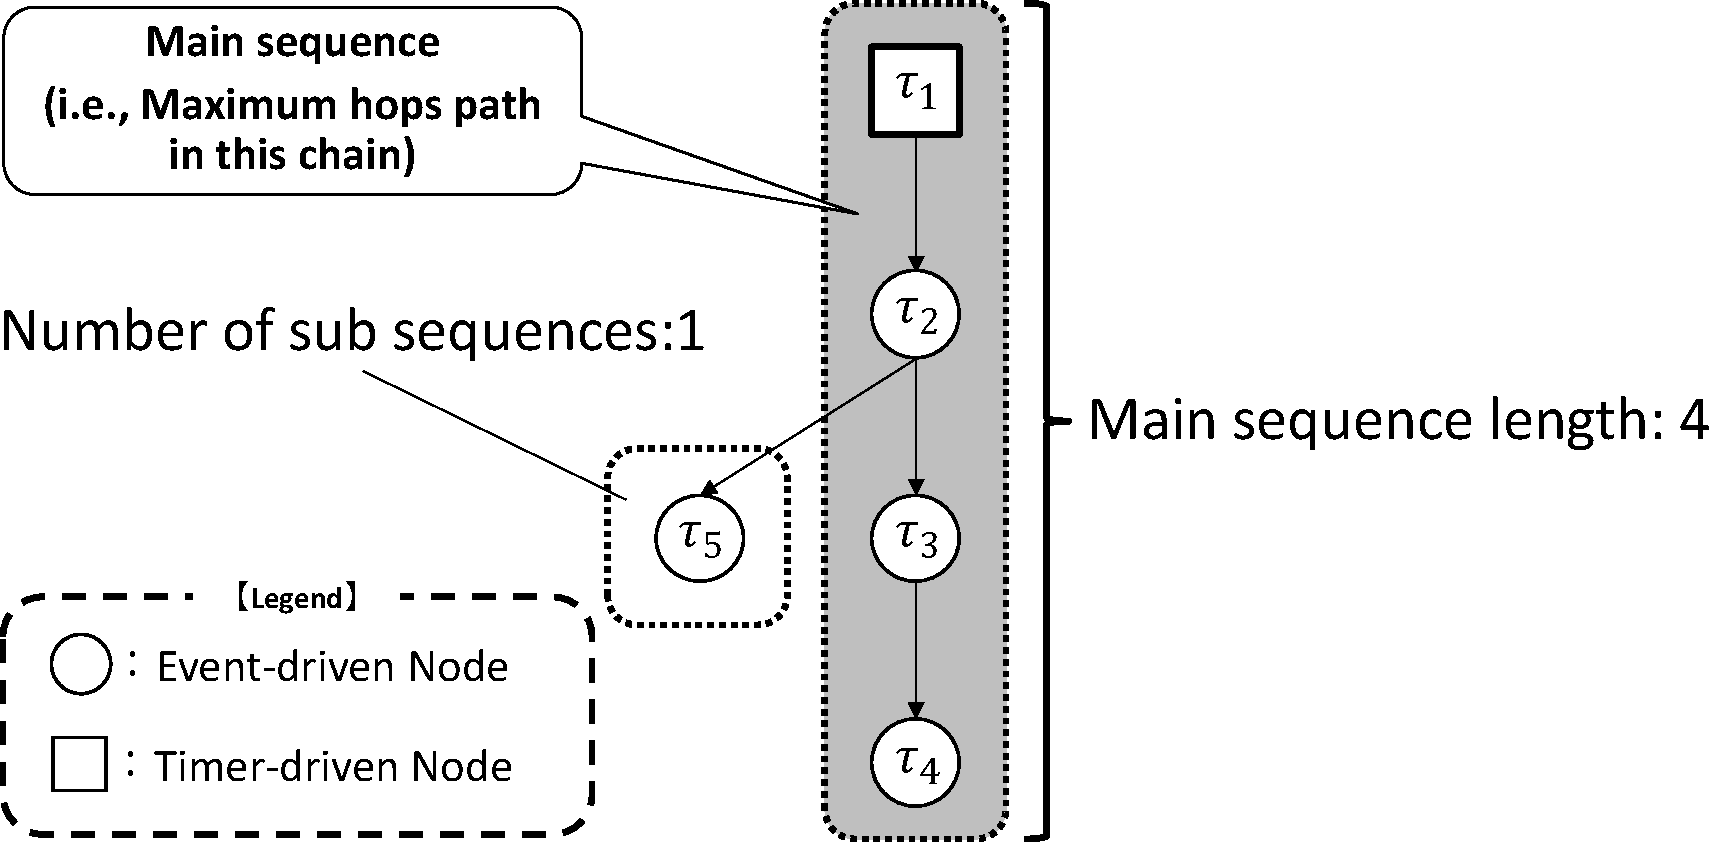
\includegraphics[width=\linewidth]{./src/figure/chain_param_exam.pdf}
    }
    \caption{Example of chain parameters}
    \label{fig: chain_param_exam}
\end{figure}


\begin{algorithm}[t]
    {\footnotesize
        \KwIn{
            $nc$ \la {\it Number of chains} \\
            $ml$ \la {\it Main sequence length} \\
            $ns$ \la {\it Number of sub sequences} \\
            $nen$ \la {\it Number of entry nodes} \\
            $nex$ \la {\it Number of exit nodes} \\
        }
        \KwOut{A DAG that satisfies user-specified parameters}
        Initialize $G$ \la $(V, E)$, with $V$ \la $\{\emptyset\}$ and $E$ \la $\{\emptyset\}$ \\
        \ForEach{$i \in 1, ..., nc$}{
            \tcc{Construct each chain}
            $main$ \la Sequence($\{\tau_{|V|+1}, ..., \tau_{|V|+ml+1}\}$) \\
            $G$ \la $main$ \\
            \ForEach{$j \in 1, ..., ns$}{
                $r$ \la Random($|V|+1, |V|+ml$) \\
                $sl$ \la Random($1, ml-r$) \\
                $sub$ \la Sequence($\{\tau_{|V|+1}, ..., \tau_{|V|+sl+1}\}$) \\
                $E$ \la $E \cup \{e_{r, |V|+1}\}$ \\
                $G$ \la $sub$ \\
            }
        }
        \tcc{Vertically link chains}
        \While{Number of entry nodes of $G$ $\neq$ $nen$}{
            $\tau_i$ \la Randomly choose one of the exit nodes in $V$ \\
            $\tau_j$ \la Randomly choose one node from the head of the chains \\
            $E$ \la $E \cup \{e_{i, j}\}$ \\
        }
        \tcc{Merge chains}
        \While{Number of exit nodes of $G$ $\neq$ $nex$}{
            $\tau_i$ \la Randomly choose one of the exit nodes in $V$ \\
            $\tau_j$ \la Randomly choose one node from other than head of the chains \\
            $E$ \la $E \cup \{e_{i, j}\}$ \\
        }
        return $G$
        \caption{{\it Chain-based} method in MRDAG-Gen}
        \label{alg: chain_based}
    }
\end{algorithm}


\subsubsection{Chain-based method}
\label{sssec: chain_based_method}

The {\it Chain-based} method is a new random DAG generation method to meet the requirements of modern chain-based multi-rate DAGs.
In the {\it Chain-based} method, multiple chains are combined to construct a single DAG.
The parameters that determine the shape of a single chain are explained here using Fig.~\ref{fig: chain_param_exam}.
The user can determine the shape of one chain by specifying {\it main sequence length} and {\it Number of subsequences}.
The main sequence is the path that has the largest number of hops from the head timer-driven node to the tail event-driven node in a single chain ($\{\tau_1, \tau_2, \tau_3, \tau_4\}$ in Fig.~\ref{fig: chain_param_exam}), and subsequences are the straight line of nodes branching off from the main sequence ($\{\tau_5\}$ in Fig.~\ref{fig: chain_param_exam}).

In the {\it Chain-based} method, two different ways of connecting chains can be specified.
The first is to link chains vertically, i.e., the event-driven node at the end of each chain is randomly connected to the timer-driven node at the head of the other chain (such as the DAG on the lower right of Fig.~\ref{fig: chain_dag}).
The second method is to integrate multiple chains in one specific node.
The {\it Chain-based} method allows nodes other than the head node of the chain to be specified as integration nodes, and the event-driven node at the tail of each chain is merged into a randomly selected integration node (such as the DAG on the upper right of Fig.~\ref{fig: chain_dag}).

The procedure of the {\it Chain-based} method is shown in Algorithm~\ref{alg: chain_based}.
First, the chains are constructed for {\it Number of chains} specified by the user (lines 2-12 in Algorithm~\ref{alg: chain_based}).
In the construction of each chain, the main sequence is first generated (lines 3-4 in Algorithm~\ref{alg: chain_based}).
Subsequences branch from random nodes other than the tail of the main sequence and are coordinated not to exceed the length of the main sequence (lines 6-10 in Algorithm~\ref{alg: chain_based}).
After all chains are generated, the chains are linked vertically until the number of entry nodes in the DAG is equal to the specified number (lines 13-17 in Algorithm~\ref{alg: chain_based}).
Finally, the chain is randomly merged until the number of exit nodes in the DAG becomes the specified number (lines 18-22 in Algorithm~\ref{alg: chain_based}).
Thus, the {\it Chain-based} method can flexibly generate DAGs consisting of multiple chains.


\begin{table*}[tb]
    \label{tab: properties}
    \caption{Properties}
    \renewcommand{\arraystretch}{1.2}
    \centering
    \scalebox{0.8}{
        \begin{tabular}{llll|l}
            \hline\hline
            \multicolumn{4}{c|}{Parameters}                 & \multicolumn{1}{c}{Descriptions}                                                                                                                                                            \\ \hline\hline
            \MC{4}{l|}{{\it Execution time}}                & Execution time of nodes                                                                                                                                                                     \\ \hline
            \MC{4}{l|}{{\it Communication time}}            & Communication time of edges                                                                                                                                                                 \\ \hline
            \MC{4}{l|}{{\it CCR}}                           & CCR of a single DAG                                                                                                                                                                         \\ \hline
            \MC{2}{l|}{{\it End-to-end deadline}}           & \MC{2}{l|}{{\it Ratio of deadline to critical path}} & Ratio of the end-to-end deadline to the critical path of DAG                                                                         \\ \hline
            \MC{2}{l|}{\MR{6}{{\it Multi-rate}}}            & \MC{2}{l|}{{\it Periodic type}}                      & Specify a group of nodes to be timer driven                                                                                          \\ \cline{3-5}
            \MC{2}{l|}{}                                    & \MC{2}{l|}{{\it Period}}                             & Period of timer-driven nodes                                                                                                         \\ \cline{3-5}
            \MC{2}{l|}{}                                    & \MC{2}{l|}{{\it Entry node period}}                  & Period of entry timer-driven nodes                                                                                                   \\ \cline{3-5}
            \MC{2}{l|}{}                                    & \MC{2}{l|}{{\it Exit node period}}                   & Period of exit timer-driven nodes                                                                                                    \\ \cline{3-5}
            \MC{2}{l|}{}                                    & \MC{2}{l|}{{\it Offset}}                             & Offset of timer-driven nodes                                                                                                         \\ \cline{3-5}
            \MC{2}{l|}{}                                    & \MC{2}{l|}{{\it Total utilization}}                  & Total utilization of a single DAG                                                                                                    \\ \hline
            \MC{2}{l|}{\MR{2}{{\it Additional properties}}} & \MC{2}{l|}{{\it Node properties}}                    & User-defined numeric parameters with any name for nodes                                                                              \\ \cline{3-5}
            \MC{2}{l|}{}                                    & \MC{2}{l|}{{\it Edge properties}}                    & User-defined numeric parameters with any name for edges                                                                              \\ \hline
            \MC{2}{l|}{\MR{9}{{\it Output formats}}}        & \MC{1}{l|}{\multirow{4}{*}{{\it DAG}}}               & {\it YAML}                                                   & \MR{4}{Outputs DAG description files in the format specified by True} \\ \cline{4-4}
            \multicolumn{2}{l|}{}                           & \multicolumn{1}{l|}{}                                & {\it JSON}                                                   &                                                                       \\ \cline{4-4}
            \multicolumn{2}{l|}{}                           & \multicolumn{1}{l|}{}                                & {\it XML}                                                    &                                                                       \\ \cline{4-4}
            \multicolumn{2}{l|}{}                           & \multicolumn{1}{l|}{}                                & {\it DOT}                                                    &                                                                       \\ \cline{3-5}
            \MC{2}{l|}{}                                    & \MC{1}{l|}{\MR{5}{{\it Figure}}}                     & {\it Draw legend}                                            & When True is specified, a legend is drawn on the output DAG figure    \\ \cline{4-5}
            \multicolumn{2}{l|}{}                           & \multicolumn{1}{l|}{}                                & {\it PNG}                                                    & \MR{4}{Outputs DAG figures in the format specified by True}           \\ \cline{4-4}
            \multicolumn{2}{l|}{}                           & \multicolumn{1}{l|}{}                                & {\it SVG}                                                    &                                                                       \\ \cline{4-4}
            \multicolumn{2}{l|}{}                           & \multicolumn{1}{l|}{}                                & {\it EPS}                                                    &                                                                       \\ \cline{4-4}
            \multicolumn{2}{l|}{}                           & \multicolumn{1}{l|}{}                                & {\it PDF}                                                    &                                                                       \\ \hline
        \end{tabular}
    }
\end{table*}


\begin{algorithm}[t]
    {\footnotesize
        \KwIn{
            $G$ \la {DAG} \\
            $pt$ \la {\it Peridoic type} \\
            $U$ \la {\it Total utilization} \\
            $p$ \la {\it Period} \\
        }
        \KwOut{A DAG that satisfies user-specified parameters}
        \If{$pt = "All"$}{
            $u[1, ..., |V|]$ \la UUniFast($|V|, U$) \cite{bini2005measuring} \\
            \ForEach{$i \in 1, ..., |V|$}{
                $T_i$ \la $p$ \\
                $C_i$ \la $u[i] \times T_i$ \\
            }
        }
        \If{$pt = "Chain"$}{
            $u[1, ..., |\Gamma|]$ \la UUniFast($|\Gamma|, U$) \\
            \ForEach{$i \in 1, ..., |\Gamma|$}{
                $T_{\Gamma_i}$ \la $p$ \\
                $C_{\Gamma_i}$ \la $u[i] \times T_{\Gamma_i}$ \\
                $g$ \la Number of nodes in $\Gamma_i$ \\
                $c[i, ..., i+g]$ \la Grouping randomly into $g$ with total equal to $C_{\Gamma_i}$ \\
                \ForEach{$j \in i, ..., i+g$}{
                    $C_j$ \la $c[j]$
                }
            }
        }
        return $G$
        \caption{Set utilization}
        \label{alg: set_utilization}
    }
\end{algorithm}


\subsection{Property setting}
\label{ssec: set_properties}

MRDAG-Gen automatically sets the typical properties that characterize the nodes and edges of a DAG to meet user requirements.
All properties that can be set automatically in MRDAG-Gen are listed in Table~\ref{tab: properties}.
MRDAG-Gen can generate (i) single-rate, (ii) multi-rate DAGs consisting of only timer-driven nodes, and (iii) chain-based multi-rate DAGs, depending on the {\it Periodic type} parameter.
If the {\it Periodic type} is not specified, DAGs of (i) are generated; if the {\it Periodic type} is {\it "All"}, DAGs of (ii) are generated; if the {\it Periodic type} is {\it "chain"}, DAGs of (iii) are generated.

In MRDAG-Gen, all properties described in Section~\ref{sec: system_model} can be specified using {\it "Fixed"}, {\it "Random"} or {\it "Combination"}.
Although existing random DAG generation tools such as TGFF and GGen provide the functionality to randomly assign properties, they do not allow the user to control the values calculated by multiple properties such as CCR and total utilization.
Since CCR and total utilization have a significant impact on the performance of scheduling algorithms and analysis methods, evaluations are performed by varying these values \cite{he2021response, agrawal2020hard, senapati2021hmds, sulaiman2021hybrid}.
Therefore, MRDAG-Gen also supports the specification of such complex property values.

An example of a property setting based on total utilization in MRDAG-Gen is shown in Algorithm~\ref{alg: set_utilization}.
MRDAG-Gen uses the UUniFast method \cite{bini2005measuring} to uniformly assign utilization to each node (lines 2 and 9 in Algorithm~\ref{alg: set_utilization}).
If the {\it Periodic type} is {\it "All"}, the utilization for each node is determined based on the {\it Total utilization} specified by the user, and the period and execution time are set to satisfy this utilization (lines 1-7 in Algorithm~\ref{alg: set_utilization}).
If the {\it Periodic type} is {\it "Chain"}, the utilization of each chain is determined based on the {\it Total utilization}, and the period of each chain and the sum of the execution time are calculated accordingly (lines 8-12 in Algorithm~\ref{alg: set_utilization}).
The total execution time is randomly divided by the number of nodes in the chain to set the execution time for each node (lines 13-17 in Algorithm~\ref{alg: set_utilization}).
In this way, MRDAG-Gen randomly and automatically sets properties according to complex parameters specified by the user.

MRDAG-Gen provides other parameters that allow for setting the ratio of end-to-end deadlines to critical path length and the period of entry and exit nodes.
In addition, users can define their unique parameters for simple properties that uniformly assign numerical values to nodes or edges.
